%========= File containing the main LaTex document ========%
%                                                          %
% Copyright (C) ISI - All Rights Reserved                  %
% Proprietary                                              %
% Written by Med Hossam <med.hossam@gmail.com>, April 2016 %
%                                                          %
% @author: HEDHILI Med Houssemeddine                       %
% @linkedin: http://tn.linkedin.com/in/medhossam           %
%==========================================================%

%\documentclass[pfe]{./tpl/isipfe}
\documentclass[]{./tpl/isipfe}
\graphicspath{{./img/}}
\usepackage{tikz}
\usetikzlibrary{positioning, arrows.meta}
\usepackage{booktabs}
\usepackage{amssymb}
\usepackage[colorlinks]{hyperref}
%\usepackage{hyperref}
% {\hypersetup{linkcolor=black}}
\input{./tpl/new_commands}
\usepackage{hyperref}
\usepackage{float}
\usepackage{listings}
\lstset{
  backgroundcolor=\color{gray!10},
  basicstyle=\ttfamily\small,
  frame=single,
  breaklines=true,       % Permet le retour à la ligne
  postbreak=\mbox{\textcolor{gray}{$\hookrightarrow$}\space}, % symbole au retour
  captionpos=b,
  xleftmargin=0.5cm,
  xrightmargin=0.5cm
}
\usepackage{enumitem}
\hypersetup{
    colorlinks = true, % Définir "true" pour activer les liens colorés
    linkcolor = black, % Définir la couleur des liens internes
    citecolor = black, % Définir la couleur des citations
    urlcolor = black   % Définir la couleur des liens URL
}
% @author: Stoufa
% the command `\makeindex` is mandatory to create the index file main.idx
% https://tex.stackexchange.com/questions/9913/input-index-file-not-found
\makeindex

\begin{document}
    
%=== File containing Global Configuration of the report ===%
%                                                          %
% Copyright (C) ISI - All Rights Reserved                  %
% Proprietary                                              %
% Written by Med Hossam <med.hossam@gmail.com>, April 2016 %
%                                                          %
% @author: HEDHILI Med Houssemeddine                       %
% @linkedin: http://tn.linkedin.com/in/medhossam           %
%==========================================================%

%=========== You MUST type your information here ==========%
% global_config.tex file is designed to configure your     %
% cover pages (main, back and black covers)                %
%==========================================================%

%============= Config new columns type ==============%
\newcolumntype{L}{>{\raggedright\arraybackslash}}
\newcolumntype{R}{>{\raggedleft\arraybackslash}}
\newcolumntype{C}{>{\centering\arraybackslash}}
%==================================================%

%========= Config the cover section ==========%

\title{Détection des Émotions Multiples dans les Textes par Fusion d'Attentions Hiérarchiques et Connaissances Sémantiques Externes  }

\author{Mariem El WEDANI}
%%% if necessary
% Set isBinomal to true and type second author name
%\setboolean{isBinomal}{true}
%\secondAuthor{Prénom NOM}


\diplomaName{Diplôme de Mastère Recherche}
\speciality{Systèmes Intelligents en Imagerie et Vision Artificielle}
%\speciality{Génie des Télécommunications et Réseaux}
%\speciality{Génie Informatique des Systèmes Industriels}

%% Encadrant professionnel
%\proFramerName{Amadou M'BODJ}
%\proFramerSpeciality{Head of Security Unit}

%% Encadrant académique
\academicFramerName{Sahbi BAHROUN}
\academicFramerSpeciality{Maître Assistant}

%% Entreprise d'accueil
%\companyName{Smart MS SA}

%% Année universitaire
\collegeYear{2025 - 2026}

%%%%%% Signatures section %%%%%%

% You can simply remove theses sentences by typing an empty string
% \proSignSentence{}

%\proSignSentence{J'autorise l'étudiante à faire le dépôt de son rapport de stage en vue d'une soutenance.}

\academicSignSentence{J'autorise l'étudiante à faire le dépôt de son rapport de stage en vue d'une soutenance.}

% %%% AR
% \arabicAbstract{}

% \arabicAbstractKeywords{}

% %% To use latin characters inside the arabic text
% % just put them inside the command \textLR{}
% %%%%

% %%% FR
% \frenchAbstract{}

% \frenchAbstractKeywords{ \\}

% %%% EN
% \englishAbstract{}

% \englishAbstractKeywords{}

%%% ARABIC
\arabicAbstract{يهدف هذا البحث إلى الكشف عن عدة مشاعر في النصوص (تصنيف متعدد التسميات) باستخدام بنية \textLR{HAKE-MER} تجمع بين الترميز الهرمي للنص، وآلية انتباه متقاطعة بين المشاعر، وإثراء دلالي بموارد خارجية. يُخطط للتقييم على مجموعة \textLR{GoEmotions} ببروتوكول إزالة تدريجية للمكونات وموازنة تدريب ثابتة.}

\arabicAbstractKeywords{كشف المشاعر، تعلم عميق، \textLR{GoEmotions}، انتباه هرمي، تصنيف متعدد التسميات}

%%% FRENCH
\frenchAbstract{Ce mémoire porte sur la détection des émotions multiples dans les textes. Nous proposons l'architecture \textLR{HAKE-MER}, combinant encodage hiérarchique, attention croisée entre émotions et enrichissement par ressources sémantiques externes. L'évaluation cible le jeu GoEmotions par ablation à protocole constant, avec un accent sur le F1-macro et les classes rares.}

\frenchAbstractKeywords{Émotions, TALN, GoEmotions, attention hiérarchique, classification multi-étiquettes}

%%% ENGLISH
\englishAbstract{This thesis addresses multi-label emotion detection in text. We propose \textLR{HAKE-MER}, combining hierarchical encoding, cross-emotion attention, and external semantic resources. Evaluation is planned on GoEmotions with controlled ablation and emphasis on macro F1 and rare emotion classes.}

\englishAbstractKeywords{Emotion detection, NLP, GoEmotions, hierarchical attention, multi-label classification}

\setboolean{wantToTypeCompanyAddress}{false}
    
    \frontmatter
        
%===== File containing the main cover of the document =====%
%                                                          %
% Copyright (C) ISI - All Rights Reserved                  %
% Proprietary                                              %
% Written by Med Hossam <med.hossam@gmail.com>, April 2016 %
%                                                          %
% @author: HEDHILI Med Houssemeddine                       %
% @linkedin: http://tn.linkedin.com/in/medhossam           %
%==========================================================%

%== It's advised to not modify the content of this file ===%
% To set your information, go to global_config.tex file    %
%==========================================================%

\thispagestyle{cover}%
\newgeometry{bottom=25mm,left=20mm,top=15mm,right=20mm}
\hspace{-47pt}
\begin{minipage}[l]{0.2\columnwidth}
\vspace{6mm}

\includegraphics[width=1.1\columnwidth]{img/logo-isi.png}\\
\end{minipage}
\hfill
\begin{minipage}[l]{0.6\columnwidth}
\centering
\footnotesize
\textbf{{République Tunisienne}}\\
\textbf{{Ministère de l'Enseignement Supérieur\\
et de la Recherche Scientifique}}\\
\textbf{{Université de Tunis El Manar}}\\
\textbf{{Institut Supérieur d'Informatique d’El Manar}}
\end{minipage}
\hfill
\begin{minipage}[l]{0.02\columnwidth}
\end{minipage}
\hfill
\begin{minipage}[l]{0.18\columnwidth}
\vspace{6mm}

\includegraphics[width=0.9\columnwidth]{Logo_UTM}\\
\end{minipage}
\vskip1.5cm

\begin{center}
{\LARGE{\textbf{Rapport de Projet de Fin d'Etudes}}}\\
\vskip0.5cm
\large

{\textbf{Présenté en vue de l'obtention du}}\\
\vskip2mm
{\textbf{\@diplomaName}}\\
{\textbf{Spécialité : \@speciality}}\\
{}
\end{center}

\begin{center}
\textrm{Par}\\
\vskip0.3cm
{\ifthenelse{\boolean{isBinomal}}
    {% IF TRUE
        \begin{center}
            \large\textbf{\@author}~~~~~ et ~~~~~
            \large\textbf{\@secondAuthor}
        \end{center}
    }
    {\Large\textbf{\@author}}% FALSE
}
\vskip12mm

\definecolor{isiBlue}{RGB}{31, 78, 121}

\begin{changemargin}{-9mm}{0cm}
\begin{minipage}[l]{1.1\columnwidth}
\begin{tcolorbox}[colframe=isiBlue,colback=white,boxrule=0pt,toprule=3pt,bottomrule=3pt,arc=0pt,top=0mm,right=0mm,left=0mm,bottom=0mm,boxsep=0.5mm]{
    \begin{tcolorbox}[colframe=isiBlue,colback=white, boxrule=0pt,toprule=1pt,bottomrule=1pt,arc=0pt,enlarge bottom by=-0.9mm, auto outer arc]
        \centering
        {\huge\textbf{\@title}}
    \end{tcolorbox}
}
\end{tcolorbox}
\end{minipage}
\end{changemargin}

\end{center}
\vskip8mm%

\begin{center}
\large
\begin{minipage}{0.92\textwidth}
\centering
\begin{tabular}{@{} >{\raggedright\arraybackslash}p{0.34\linewidth}
                  >{\centering\arraybackslash}p{0.38\linewidth}
                  >{\raggedleft\arraybackslash}p{0.24\linewidth} @{}}
Encadrant académique : & \textbf{\@academicFramerName} & \@academicFramerSpeciality \\
\end{tabular}
\end{minipage}
\end{center}
\vskip16mm

% \begin{center}
% \large
% Réalisé au sein de \@companyName\\
% \vskip0.4cm
% \begin{figure}[h]
% \centering
% {\color{isiBlue}{\fboxrule=2.5pt\fbox{
\includegraphics[width=0.4\columnwidth]{img/logo_smart.png}}}}
% \end{figure}
% \end{center}

% \afterpage{\blankpage}
        \include{tpl/cover_page_black}
        \input{tpl/signatures}
        
        \setcounter{page}{0
        }
        % \chapter*{\Huge \textit{Dédicaces}}

\begingroup
\large \raggedright
\begin{center}
    

\textit{
Je dédie ce travail, avant tout, à ma mère bien-aimée \textbf{Raghiya ISSA}, pour son amour infini, ses prières constantes et ses sacrifices silencieux.}\\

\textit{À mes chères sœurs, avec une pensée particulière pour \textbf{Kertouma MOUSSA}, et à mes frères, pour leur affection, leur soutien moral et leur encouragement inébranlable.}\\

\textit{À mes amis fidèles, pour leur présence rassurante durant les moments difficiles, et plus spécialement à Moulay Abderrahmane SIDATTY, pour son amitié sincère, sa patience, ses conseils avisés et son soutien précieux tout au long de ce parcours.}\\

\textit{À tous les membres de ma famille, à mes parents dans le sens le plus large, et à toutes les personnes bienveillantes qui ont, de près ou de loin, contribué à la réussite de ce projet.}\\
\end{center}
\endgroup

\vspace{8mm}
\begin{flushright}
    \LARGE \textbf{\@author}
\end{flushright}

        % \thispagestyle{frontmatter}
        % \chapter*{\huge Remerciements}
\noindent Avant toute chose, je rends grâce à Dieu — \textit{Al Hamdoulilah} — pour m’avoir donné la force, la patience et la persévérance nécessaires à l’accomplissement de ce travail.

\noindent Je tiens à exprimer mes plus sincères remerciements à toutes les personnes qui ont contribué, de près ou de loin, à la réalisation de ce projet de fin d’études. Leur soutien, leurs conseils et leur bienveillance m’ont été d’une aide précieuse tout au long de cette aventure. Qu’elles trouvent ici l’expression de ma profonde gratitude.

\noindent Je remercie tout d’abord :
\begin{itemize}[label=\textbullet]
\item \textbf{SMART MS SA}, pour m’avoir offert l’opportunité d’effectuer ce stage dans un environnement professionnel stimulant et enrichissant.
\item \textbf{L’Institut Supérieur d’Informatique (ISI)}, pour la qualité de sa formation et l’encadrement académique rigoureux dont j’ai bénéficié tout au long de mon cursus.
\end{itemize}

\noindent Je souhaite remercier tout particulièrement :
\begin{itemize}[label=\textbullet]
\item \textbf{Monsieur Amadou M’Bodj}, professionnel chez SMART MS, pour sa supervision technique, sa pédagogie et les nombreuses compétences qu’il m’a aidé à développer.
\item \textbf{Monsieur Sahbi Bahroun}, mon encadrant académique, pour son accompagnement, sa disponibilité et ses conseils avisés tout au long de ce projet.
\vspace{0.6cm}
\end{itemize}
Enfin, j’exprime toute ma reconnaissance à mes parents, pour leur amour inconditionnel, leurs sacrifices et leur soutien indéfectible tout au long de mon parcours. Je remercie également l’ensemble des enseignants de l’ISI pour la qualité de leur enseignement et leur engagement, ainsi que toutes les familles et personnes bienveillantes qui m’ont soutenue durant ma formation. Une pensée particulière va à mon oncle, \textbf{Monsieur Souleyman Diallo}, pour son appui constant, et à mon oncle, \textbf{Dr. Mohamed El Wedani (Bouyati)}, pour ses encouragements et l’inspiration qu’il m’a toujours apportée. Je tiens aussi à remercier mon camarade et ami, l’ingénieur \textbf{Moulay Abderrahmane Sidatty}, pour sa présence précieuse, ses conseils et son soutien inestimable durant les moments les plus décisifs de mon parcours.


        % \thispagestyle{frontmatter}
        
        \setcounter{secnumdepth}{3}
        \setcounter{tocdepth}{2}
        \dominitoc
        \hypersetup{linkcolor=black}\tableofcontents
        \adjustmtc
        \thispagestyle{frontmatter}
        
        \listoffigures
        \thispagestyle{frontmatter}
        \listoftables
        \thispagestyle{frontmatter}
        
        % \chapter*{Liste des abréviations}

%=============== Glossary example ==============%
% it's an enhanced itemize list to make it      %
% sortable automatically.                       %
%===============================================%

\begin{itemize}[label=\textbullet]
    \item \textbf{ACL} : \textbf{A}ccess \textbf{C}ontrol \textbf{L}ist
    \item \textbf{AD} : \textbf{A}ctive \textbf{D}irectory
    \item \textbf{AD DS} : \textbf{A}ctive \textbf{D}irectory \textbf{D}omain \textbf{S}ervices
    \item \textbf{API RESTful} : \textbf{A}pplication \textbf{P}rogramming \textbf{I}nterface (\textbf{RE}presentational \textbf{S}tate \textbf{T}ransfer)
    \item \textbf{APT} : \textbf{A}dvanced \textbf{P}ersistent \textbf{T}hreat
    \item \textbf{BYOD} : \textbf{B}ring \textbf{Y}our \textbf{O}wn \textbf{D}evice
    \item \textbf{CIA} : \textbf{C}onfidentiality, \textbf{I}ntegrity, \textbf{A}vailability
    \item \textbf{CISO} : \textbf{C}hief \textbf{I}nformation \textbf{S}ecurity \textbf{O}fficer
    \item \textbf{CPU} : \textbf{C}entral \textbf{P}rocessing \textbf{U}nit
    \item \textbf{DAC} : \textbf{D}iscretionary \textbf{A}ccess \textbf{C}ontrol
    \item \textbf{DC} : \textbf{D}omain \textbf{C}ontroller
    \item \textbf{DDoS} : \textbf{D}istributed \textbf{D}enial \textbf{o}f \textbf{S}ervice
    \item \textbf{DFIR} : \textbf{D}igital \textbf{F}orensics and \textbf{I}ncident \textbf{R}esponse
    \item \textbf{DNS} : \textbf{D}omain \textbf{N}ame \textbf{S}ystem
    \item \textbf{DoS} : \textbf{D}enial \textbf{of} \textbf{S}ervice
    \item \textbf{DCSync} : \textbf{D}irectory \textbf{C}ontroller \textbf{Sync}hronization
    \item \textbf{EDR} : \textbf{E}ndpoint \textbf{D}etection and \textbf{R}esponse
    \item \textbf{EICAR} : \textbf{E}uropean \textbf{I}nstitute for \textbf{C}omputer \textbf{A}ntivirus \textbf{R}esearch
    \item \textbf{ELK} : \textbf{E}lasticsearch, \textbf{L}ogstash, \textbf{K}ibana
    \item \textbf{EPP} : \textbf{E}ndpoint \textbf{P}rotection \textbf{P}latform
    \item \textbf{FSMO} : \textbf{F}lexible \textbf{S}ingle \textbf{M}aster \textbf{O}peration
    \item \textbf{GPMC} : \textbf{G}roup \textbf{P}olicy \textbf{M}anagement \textbf{C}onsole
    \item \textbf{GPO} : \textbf{G}roup \textbf{P}olicy \textbf{O}bject
    \item \textbf{HIPAA} : \textbf{H}ealth \textbf{I}nsurance \textbf{P}ortability and \textbf{A}ccountability \textbf{A}ct
    \item \textbf{HTML} : \textbf{H}yper\textbf{T}ext \textbf{M}arkup \textbf{L}anguage
    \item \textbf{HTTP} : \textbf{H}yper\textbf{T}ext \textbf{T}ransfer \textbf{P}rotocol
    \item \textbf{IA} : \textbf{I}ntelligence \textbf{A}rtificielle
    \item \textbf{IDS} : \textbf{I}ntrusion \textbf{D}etection \textbf{S}ystem
    \item \textbf{IP} : \textbf{I}nternet \textbf{P}rotocol
    \item \textbf{ISO} : \textbf{I}nternational \textbf{O}rganization for \textbf{S}tandardization
    \item \textbf{ITDR} : \textbf{I}dentité \textbf{T}hreat \textbf{D}etection and \textbf{R}esponse
    \item \textbf{ITIL} : \textbf{I}nformation \textbf{T}echnology \textbf{I}nfrastructure \textbf{L}ibrary
    \item \textbf{JSON} : \textbf{J}avaScript \textbf{O}bject \textbf{N}otation
    \item \textbf{KDC} : \textbf{K}ey \textbf{D}istribution \textbf{C}enter
    \item \textbf{LDAP} : \textbf{L}ightweight \textbf{D}irectory \textbf{A}ccess \textbf{P}rotocol
    \item \textbf{LLMNR/NBT-NS} : \textbf{L}ink-\textbf{L}ocal \textbf{M}ulticast \textbf{N}ame \textbf{R}esolution / \textbf{N}et\textbf{B}IOS over \textbf{T}CP-\textbf{N}ame \textbf{S}ervice
    \item \textbf{LSA} : \textbf{L}ocal \textbf{S}ecurity \textbf{A}uthority
    \item \textbf{MAC} : \textbf{M}andatory \textbf{A}ccess \textbf{C}ontrol
    \item \textbf{MFA} : \textbf{M}ulti-\textbf{F}actor \textbf{A}uthentication
    \item \textbf{MITM} : \textbf{M}an \textbf{I}n \textbf{T}he \textbf{M}iddle
    \item \textbf{MITRE ATT\&CK} : \textbf{M}ITRE \textbf{Adversarial T}actics, \textbf{T}echniques, and \textbf{C}ommon \textbf{K}nowledge
    \item \textbf{NTLM} : \textbf{N}ew \textbf{T}echnology \textbf{L}AN \textbf{M}anager
    \item \textbf{OU} : \textbf{O}rganizational \textbf{U}nit
    \item \textbf{PCA} : \textbf{P}lan de \textbf{C}ontinuité \textbf{d'}\textbf{A}ctivité
    \item \textbf{PCI-DSS} : \textbf{P}ayment \textbf{C}ard \textbf{I}ndustry – \textbf{D}ata \textbf{S}ecurity \textbf{S}tandard
    \item \textbf{PRA} : \textbf{P}lan de \textbf{R}eprise \textbf{d'}\textbf{A}ctivité
    \item \textbf{RBAC} : \textbf{R}ole-\textbf{B}ased \textbf{A}ccess \textbf{C}ontrol
    \item \textbf{RAM} : \textbf{R}andom \textbf{A}ccess \textbf{M}emory
    \item \textbf{SAM} : \textbf{S}ecurity \textbf{A}ccount \textbf{M}anager
    \item \textbf{SID} : \textbf{S}ecurity \textbf{I}dentifier
    \item \textbf{SI} : \textbf{S}écurité \textbf{I}nformatique
    \item \textbf{SIEM} : \textbf{S}ecurity \textbf{I}nformation and \textbf{E}vent \textbf{M}anagement
    \item \textbf{SIM} : \textbf{S}ystème d'\textbf{I}nformation \textbf{M}anagé
    \item \textbf{SMB} : \textbf{S}erver \textbf{M}essage \textbf{B}lock
    \item \textbf{SOAR} : \textbf{S}ecurity \textbf{O}rchestration, \textbf{A}utomation and \textbf{R}esponse
    \item \textbf{SPN} : \textbf{S}ervice \textbf{P}rincipal \textbf{N}ame
    \item \textbf{SQL} : \textbf{S}tructured \textbf{Q}uery \textbf{L}anguage
    \item \textbf{SSL} : \textbf{S}ecure \textbf{S}ockets \textbf{L}ayer
    \item \textbf{TCP} : \textbf{T}ransmission \textbf{C}ontrol \textbf{P}rotocol
    \item \textbf{TGS} : \textbf{T}icket \textbf{G}ranting \textbf{S}ervice
    \item \textbf{TGT} : \textbf{T}icket \textbf{G}ranting \textbf{T}icket
    \item \textbf{TIC} : \textbf{T}echnologies de l'\textbf{I}nformation et de la \textbf{C}ommunication
    \item \textbf{TLS} : \textbf{T}ransport \textbf{L}ayer \textbf{S}ecurity
    \item \textbf{TTP} : \textbf{T}actics, \textbf{T}echniques, and \textbf{P}rocedures
    \item \textbf{VM} : \textbf{V}irtual \textbf{M}achine
    \item \textbf{VPN} : \textbf{V}irtual \textbf{P}rivate \textbf{N}etwork
    \item \textbf{XML} : \textbf{E}xtensible \textbf{M}arkup \textbf{L}anguage
    
    
\end{itemize}

        % \thispagestyle{frontmatter}
    
    \mainmatter
        \chapter*{Introduction générale}
\addcontentsline{toc}{chapter}{Introduction générale}
\markboth{Introduction générale}{}

Les textes produits en ligne (commentaires, messages, avis) véhiculent
des états affectifs qui dépassent souvent une simple polarité positive ou
négative. La \textbf{détection d'émotions} vise à identifier des catégories
affectives fines (joie, colère, tristesse, peur, etc.), fréquemment
\textbf{plusieurs à la fois} dans un même énoncé. Cette tâche relève de la
classification \emph{multi-étiquettes} : chaque émotion est une décision
binaire, et les cooccurrences ainsi que le \textbf{déséquilibre} des classes
: quelques labels très fréquents, beaucoup d'autres rares, compliquent
l'apprentissage et l'évaluation.

Ce mémoire s'inscrit dans le Mastère de Recherche à l'Institut Supérieur
d'Informatique (ISI), sous l'encadrement de M.~Sahbi Bahroun. Il porte sur
la conception de \textbf{HAKE-MER} (\emph{Hierarchical Attention with
Knowledge Enhancement for Multi-Emotion Recognition}), une architecture
modulaire destinée à mieux exploiter la \textbf{structure} du texte
(phrases, document), les \textbf{interactions entre émotions}, et des
\textbf{ressources sémantiques externes} (lexiques affectifs). L'évaluation s'appuie sur le corpus GoEmotions \cite{demszky2020},
référence pour les émotions fines en anglais, avec un protocole d'ablation à
budget d'entraînement constant et le \textbf{F1-macro} comme métrique
principale. Les campagnes Step~0 à M4 sont exécutées sur DistilBERT-base
(chapitre~\ref{chap:experimentation}) ; RoBERTa ne couvre que le Step~0 flat.

\textbf{Contributions de ce mémoire} :
\begin{itemize}[noitemsep]
\item une architecture en quatre modules cumulables (encodage hiérarchique,
      attention croisée, enrichissement lexical, pondération dynamique) ;
\item un protocole expérimental explicite (hypothèses H1 à H4, deux backbones
      pré-entraînés, comparaison NRC / SenticNet) ;
\item une analyse visant les performances \emph{par classe}, au-delà des
      moyennes globales.
\end{itemize}

Ce rapport enchaîne problématique, état de l'art, conception et
résultats quantitatifs : le chapitre~\ref{chap:experimentation} reporte
les métriques test et tranche H1 à H4.

\paragraph{Organisation du mémoire.}
Le chapitre~\ref{chap:contexte} présente le contexte, la problématique et
les objectifs. Le chapitre~\ref{chap:etat_art} situe HAKE-MER par rapport
à la littérature sur les émotions multiples, l'attention hiérarchique et
l'intégration de connaissances. Le chapitre~\ref{chap:conception} détaille
l'architecture et les hypothèses de recherche. Le
chapitre~\ref{chap:experimentation} fixe le cadre expérimental. Le
chapitre~\ref{chap:perspectives} discute recommandations et prolongements.
Une conclusion générale clôt le document.

        \clearpage
        
        \chapter{Contexte général et problématique}
\label{chap:contexte}

\section*{Introduction}
\addcontentsline{toc}{section}{Introduction}

Ce chapitre introduit le contexte scientifique et les motivations du présent
travail sur la détection des émotions multiples dans les textes. Il commence
par situer le cadre institutionnel du projet, avant de formuler la
problématique de recherche. Les objectifs et les questions de recherche qui
en découlent sont ensuite présentés, puis le chapitre se conclut par la
description du plan de travail adopté, qui structure la démarche
méthodologique suivie tout au long du mémoire.

\section{Cadre général du projet}
\label{sec:cadre-general}

Ce travail s'inscrit dans le cadre du Projet de Fin d'Études du Mastère de
Recherche en Informatique, spécialité Sciences et Technologies de
l'Information, réalisé à l'Institut Supérieur d'Informatique (ISI) de
l'Université de Tunis El Manar, sous l'encadrement du Dr.~Sahbi Bahroun. Le
sujet porte sur la conception d'une architecture neuronale pour la
détection des émotions multiples dans les textes, combinant attention
hiérarchique et connaissances sémantiques externes.

L'analyse automatique des émotions dans le texte s'est imposée comme un
sous-domaine central du traitement automatique des langues, avec des
applications directes en modération de contenu, en analyse de l'expérience
client, en santé mentale numérique et en systèmes conversationnels
affectifs. Contrairement à l'analyse de sentiment classique, qui réduit un
texte à une polarité (positif, négatif, neutre) \cite{pang2008,mohammad2020sentiment},
la détection d'émotions vise à identifier des catégories affectives fines
(joie, colère, tristesse, surprise, etc.), souvent multiples et simultanées
au sein d'un même énoncé.

\section{Problématique}
\label{sec:problematique}

La plupart des travaux en classification des émotions textuelles reposent
sur l'hypothèse simplificatrice qu'un texte exprime une émotion dominante
unique. Cette hypothèse ne reflète pas la réalité des
états affectifs humains, qui se manifestent fréquemment sous forme de
mélanges d'émotions coexistant dans un même énoncé, par exemple
l'expression simultanée de la surprise et de la joie, ou de la déception et
de la colère. Les jeux de données récents à annotation multi-étiquettes,
tels que GoEmotions \cite{demszky2020}, montrent qu'environ 17\,\% des
textes portent au moins deux émotions simultanées, ce qui invalide
l'approche mono-étiquette pour un grand nombre de cas réels.

Trois limites structurelles freinent les approches existantes de
détection multi-émotions, détaillées et documentées au chapitre~2 :

\begin{itemize}
\item \textbf{L'indépendance supposée des étiquettes.} Les architectures de
  classification multi-label standards traitent chaque émotion comme une
  décision binaire indépendante, ignorant les corrélations et
  incompatibilités entre émotions (la joie et la tristesse sont rarement
  co-actives, tandis que la surprise accompagne souvent la peur ou la
  joie).
\item \textbf{La perte de la structure du texte.} L'encodage global d'un
  texte en un unique vecteur de représentation efface les signaux
  localisés à l'échelle de la phrase, alors que dans les textes
  multi-phrases, différentes émotions sont souvent portées par des
  segments distincts du texte.
\item \textbf{Le déséquilibre sévère des classes.} La distribution des
  émotions dans les corpus réels suit une loi de puissance : quelques
  émotions fréquentes (joie, neutralité) dominent très largement les
  émotions rares (deuil, soulagement, nervosité), ce qui pénalise
  l'apprentissage des classes minoritaires, précisément celles pour
  lesquelles la détection est la plus critique en pratique.
\end{itemize}

Ces limites motivent la question de recherche centrale de ce mémoire :
\textit{dans quelle mesure une architecture combinant encodage
hiérarchique, attention croisée entre émotions et enrichissement par
connaissances sémantiques externes peut-elle améliorer la détection des
émotions rares et multiples dans le texte, par rapport à un modèle
pré-entraîné affiné de façon standard ?}

\section{Objectifs de recherche}
\label{sec:objectifs}

Pour répondre à cette question, ce travail poursuit les objectifs suivants :

\begin{itemize}
\item \textbf{Concevoir} une architecture modulaire, HAKE-MER, structurée
  en quatre composantes cumulables (encodage hiérarchique, attention
  croisée multi-émotions, enrichissement sémantique, pondération
  dynamique), permettant d'isoler la contribution de chaque mécanisme ;
\item \textbf{Évaluer} cette architecture de façon rigoureuse sur le jeu de
  données GoEmotions, par un protocole d'ablation cumulative à budget
  d'entraînement strictement constant, sur deux backbones pré-entraînés
  (DistilBERT et RoBERTa), afin de garantir que les gains observés sont
  attribuables aux composantes architecturales et non à des facteurs
  confondus ;
\item \textbf{Comparer} deux ressources de connaissances externes de nature
  différente (lexique catégoriel NRC contre ressource conceptuelle
  SenticNet) afin de déterminer laquelle s'intègre le mieux à
  l'architecture proposée ;
\item \textbf{Analyser} les résultats au niveau de la classe, au-delà des
  métriques globales, pour évaluer l'apport réel de chaque composante sur
  les émotions rares, enjeu applicatif central du sujet.
\end{itemize}

\section{Plan de travail}
\label{sec:plan-travail}

La démarche suivie dans ce mémoire s'inspire d'un processus itératif de
type CRISP-DM (Cross-Industry Standard Process for Data Mining), adapté au
contexte d'un projet de recherche en apprentissage profond. Le
Tableau~\ref{tab:plan-travail} résume les phases méthodologiques adoptées.

\begin{table}[H]
\centering
\caption{Phases méthodologiques du plan de travail}
\label{tab:plan-travail}
\begin{tabular}{|p{4cm}|p{9cm}|}
\hline
\textbf{Phase} & \textbf{Contenu} \\
\hline
Analyse du problème et revue de littérature &
Formulation de la problématique, revue critique des approches de
détection multi-émotions, d'attention hiérarchique et d'intégration de
connaissances externes (chapitre~2), identification du positionnement de
HAKE-MER. \\
\hline
Compréhension et préparation des données &
Exploitation des statistiques GoEmotions (chapitre~2), choix du
prétraitement et de la longueur de séquence. \\
\hline
Conception et modélisation &
Formulation du problème, conception de l'architecture HAKE-MER et de ses
quatre modules, définition des hypothèses de recherche H1 à H4
(chapitre~3). \\
\hline
Expérimentation et évaluation &
Implémentation, protocole d'ablation à budget constant (Step~0 sur
DistilBERT et RoBERTa ; ladder M1 à M4 sur DistilBERT), comparaison
NRC/SenticNet, analyse par classe (chapitre~4). \\
\hline
Documentation et valorisation &
Rédaction du mémoire, synthèse des enseignements méthodologiques et des
recommandations pratiques (chapitre~5), structuration de l'état de
l'art en survey autonome en vue d'une valorisation après soutenance. \\
\hline
\end{tabular}
\end{table}

\section*{Conclusion}
\addcontentsline{toc}{section}{Conclusion}

Ce premier chapitre a présenté le cadre général du projet, formulé la
problématique de la détection des émotions multiples dans les textes et
défini les objectifs de recherche qui en découlent, ainsi que le plan de
travail du mémoire. Pour rendre la question centrale opérationnelle, il
reste à fixer la tâche et le corpus de référence, à identifier une
baseline crédible et à examiner comment la littérature répond aux
limitations L1 à L3 (étiquettes, structure du texte, classes rares) avant
de positionner HAKE-MER ; c'est l'objet du chapitre~2.

        \clearpage

        \chapter{État de l'art}
\label{chap:etat_art}

\section*{Introduction}
La compréhension automatique des émotions humaines dans le texte constitue l'un des défis centraux du Traitement Automatique du Langage Naturel (TALN). Longtemps abordée comme un problème de classification mono-étiquette visant à identifier l'émotion dominante d'un énoncé, la détection des émotions connaît aujourd'hui un tournant paradigmatique : la réalité du langage humain révèle que plusieurs émotions peuvent coexister simultanément dans un même texte, s'interpénétrer, se moduler et interagir à différentes granularités linguistiques.

\noindent Le présent travail s'inscrit dans ce contexte en proposant l'architecture \textbf{HAKE-MER} (\textit{Hierarchical Attention with Knowledge Enhancement for Multi-Emotion Recognition}), une approche qui ambitionne de dépasser les limitations des méthodes existantes en combinant : \\
(i) une modélisation hiérarchique multi-niveaux basée sur les transformers \cite{vaswani2017,devlin2019,yang2016}, \\
(ii) un mécanisme d'attention croisée pour capturer les interactions inter-émotions,\\
(iii) une intégration de connaissances sémantiques externes issues de bases telles que \textit{ConceptNet} \cite{speer2017} et \textit{EmoNet}.

\noindent Le présent état de l'art explore les cinq axes thématiques suivantes : les méthodes de détection d'émotions multiples, les architectures d'attention hiérarchique et les transformers, l'intégration de connaissances externes, les techniques de raisonnement par bon sens, et les approches d'apprentissage multi-niveaux et multi-granularités.

\section{Méthodes de Détection d'Émotions Multiples (Multi-label Emotion Classification)}

\subsection{Fondements et cadrage du problème}
\noindent La détection des émotions dans le texte s'appuie historiquement sur deux théories fondatrices : la théorie des émotions de base d'Ekman (1992), qui postule l'existence de six émotions universelles (joie, tristesse, peur, colère, dégoût, surprise), et la théorie dimensionnelle de Russell (1980), fondée sur un espace bidimensionnel valence-arousal (V-A). Ces deux approches ont structuré les premiers systèmes de classification, mais leurs limitations sont manifestes dès lors que l'on confronte la richesse émotionnelle du langage naturel à ces catégories rigides.

\noindent La classification multi-étiquettes (\textit{multi-label classification}, MLC) constitue le cadre formel adapté à la détection simultanée de plusieurs émotions. Formellement, étant donné un énoncé $x$ et un ensemble d'étiquettes émotionnelles $L = \{l_{1}, l_{2}, \dots, l_{n}\}$, la tâche consiste à apprendre une fonction
\[
f : x \rightarrow \{0,1\}^{n}
\]
assignant à chaque étiquette une valeur binaire ou un score de probabilité. Cette formulation diffère fondamentalement de la classification multi-classes, où une seule étiquette est attribuée.

\subsection{Approches basées sur les features classiques}
\noindent Les premières approches de classification émotionnelle multi-étiquettes reposaient sur l'extraction manuelle de traits linguistiques : n-grammes, présence de mots affectifs issus de lexiques (\textit{LIWC}, \textit{SentiWordNet}, \textit{NRC Emotion Lexicon}), structures syntaxiques et traits prosodiques. Ces représentations étaient ensuite classifiées par des algorithmes tels que les \textit{Support Vector Machines} (SVM) en configuration multi-label, les forêts aléatoires, ou les chaînes de classificateurs (\textit{Classifier Chains}) de Read et al. (2009), qui modélisent explicitement les dépendances entre étiquettes.

\noindent La limite majeure de ces méthodes réside dans leur incapacité à capturer la sémantique profonde et les dépendances contextuelles à longue portée, ainsi que leur fragilité face aux expressions figuratives, à l'ironie et aux émotions implicites.

\subsection{Approches par apprentissage profond}
\noindent L'avènement du deep learning a profondément reconfiguré le paysage de la détection émotionnelle multi-étiquettes. Les réseaux convolutionnels (CNN) de Kim (2014) ont démontré l'efficacité des filtres locaux pour la classification de textes courts. Les réseaux récurrents bidirectionnels (BiLSTM) ont ensuite permis de capturer les dépendances séquentielles dans les deux sens de lecture, surpassant les CNN sur des tâches nécessitant une compréhension contextuelle étendue.

\noindent Un apport méthodologique majeur dans le contexte multi-label est le mécanisme d'attention de Bahdanau et al. (2015) \cite{bahdanau2015}, qui permet au modèle de pondérer différemment les tokens selon leur pertinence pour chaque étiquette. Des extensions telles que l'attention spécifique à une étiquette (\textit{label-specific attention}) ont été proposées pour modéliser individuellement la contribution de chaque région textuelle à chaque émotion.

\subsection{Défis spécifiques : labellisation incomplète et subjectivité}
\noindent La construction de datasets pour la détection multi-émotions est confrontée à deux problèmes structurels majeurs. D'une part, la labellisation incomplète (\textit{partial label learning}) : les annotateurs tendent à ne marquer que les émotions saillantes, omettant les émotions de faible intensité ou secondaires. D'autre part, la subjectivité inhérente à la perception émotionnelle fait que différents annotateurs peuvent attribuer des étiquettes contradictoires au même énoncé.

\noindent Des approches de \textit{learning with noisy labels}, d'agrégation bayésienne des annotations (Dawid \& Skene, 1979 ; Rodrigues \& Pereira, 2018) et de \textit{curriculum learning} ont été proposées pour atténuer ces biais. La modélisation probabiliste des distributions d'étiquettes plutôt que des affectations binaires constitue une direction prometteuse explorée notamment par Demszky et al. (2020) dans la conception du dataset \textit{GoEmotions} \cite{demszky2020}.

\section{Architectures d'Attention Hiérarchique et Transformers}

\subsection{Le mécanisme d'attention : fondements théoriques}
\noindent Le mécanisme d'attention, introduit formellement par Bahdanau et al. (2015) \cite{bahdanau2015} dans le cadre des modèles séquence-à-séquence, puis généralisé sous la forme d'une attention multi-têtes (\textit{multi-head attention}) par Vaswani et al. (2017) \cite{vaswani2017} dans l'architecture \textit{Transformer}, constitue le socle théorique des approches modernes de TALN. L'attention permet à un modèle de calculer, pour chaque position d'une séquence, une pondération sur l'ensemble des autres positions, capturant ainsi des dépendances arbitrairement longues sans les limitations des architectures récurrentes.

Formellement, l'attention est calculée comme :
\[
\text{Attention}(Q,K,V)=\text{softmax}\left(\frac{QK^{T}}{\sqrt{d_k}}\right)V
\]
où $Q$, $K$, $V$ désignent respectivement les matrices \textit{query}, \textit{key} et \textit{value}, et $d_k$ est la dimension des clés. Cette formulation est au cœur de l'architecture \textit{Transformer} et de tous ses descendants \cite{vaswani2017}.

\subsection{L'architecture Transformer et ses variants pré-entraînés}
\noindent L'architecture \textit{Transformer} \cite{vaswani2017} a engendré une famille de modèles pré-entraînés sur de larges corpus textuels, qui ont révolutionné pratiquement toutes les tâches de TALN. BERT \cite{devlin2019} introduit un pré-entraînement bidirectionnel par masquage de tokens (\textit{Masked Language Modeling}) et prédiction de phrase suivante, produisant des représentations contextuelles riches. RoBERTa (Liu et al., 2019) améliore BERT par un entraînement plus long sur un corpus plus large et la suppression de la tâche NSP. XLNet (Yang et al., 2019) adopte un schéma autorégressif permutationnel contournant les limitations du masquage.

\noindent Pour le domaine affectif, des variantes spécialisées ont été développées : RoBERTa-base fine-tuné sur des datasets émotionnels \cite{demszky2020}, SentiBERT (Yin et al., 2020) enrichi de structures syntaxiques, et EmotionBERT. Ces modèles constituent les encodeurs de base des approches \textit{state-of-the-art} pour la classification émotionnelle multi-étiquettes.

\subsection{Architectures d'attention hiérarchique}
\noindent La modélisation hiérarchique du texte vise à capturer les structures à différentes granularités : mot, phrase (ou clause), et document. Le \textit{Hierarchical Attention Network} (HAN) proposé par Yang et al. (2016) \cite{yang2016} pour la classification de documents constitue le modèle fondateur de cette famille d'approches. HAN empile deux niveaux d'encodeurs BiGRU avec attention : un au niveau des mots au sein de chaque phrase, et un au niveau des phrases au sein du document, permettant de capturer la structure rhétorique du texte.

\noindent Des extensions hiérarchiques des transformers ont ensuite été proposées pour traiter des textes longs. Le modèle HIBERT (Zhang et al., 2019) applique des encodeurs transformer à deux niveaux. Des architectures récentes comme HAT (\textit{Hierarchical Attention Transformer}) utilisent des self-attentions locales au niveau des segments et une attention globale au niveau du document, réduisant la complexité computationnelle tout en maintenant une modélisation multi-échelle.

\noindent Dans le contexte émotionnel spécifique, Luo et al. (2025) proposent un mécanisme d'attention à trois dimensions pour la classification multi-étiquettes des émotions : une couche d'attention distincte par émotion, chacune traitée comme un plan bidimensionnel, reliées entre elles par une attention multi-têtes, avec un paramètre de polarité/intensité (\textit{Commander}) modulant les poids d'attention. Évaluée sur \textit{GoEmotions} et \textit{SemEval-2018}, cette approche porte le F1-macro de 0,46 à 0,56 sur GoEmotions \cite{luo2025attention}. Dans un cadre plus général de classification multi-étiquettes, Li et al. (2022) proposent une architecture Transformer-CNN hiérarchique combinant une attention multi-têtes au niveau des mots et un CNN au niveau des phrases pour capturer l'information sémantique à plusieurs échelles \cite{li2022hierarchical} ; bien que non spécifique aux émotions, ce principe de traitement hiérarchique multi-échelle rejoint directement la motivation du module d'encodage hiérarchique de HAKE-MER.

\subsection{Attention croisée pour les interactions entre émotions}
\noindent La modélisation des interactions entre émotions constitue un verrou scientifique central. Les émotions ne sont pas indépendantes : la joie et la surprise sont fréquemment co-occurrentes, tandis que la joie et la tristesse s'excluent plus souvent. Des mécanismes d'attention croisée (\textit{cross-attention}) ou d'attention inter-étiquettes permettent de capturer ces corrélations. Des approches comme le \textit{Label-Correlation Attention} de Chen et al. (2023) construisent un graphe d'émotions et appliquent des réseaux d'attention sur ce graphe pour propager les signaux entre étiquettes corrélées.

\section{Intégration de Connaissances Externes}

\subsection{Motivation et cadre général}
\noindent L'intégration de connaissances externes dans les modèles de TALN répond à une limitation fondamentale des approches purement statistiques : la difficulté à inférer les émotions implicites, à comprendre les références culturelles ou à désambiguïser les expressions indirectes. Les connaissances structurées permettent d'ancrer les représentations dans une sémantique explicite et d'effectuer des inférences au-delà de la co-occurrence statistique.

\subsection{Bases de connaissances affectives}
\noindent Plusieurs ressources sémantiques ont été développées pour le domaine affectif. NRC Emotion Lexicon (Mohammad \& Turney, 2013) associe plus de 14\,000 mots à huit catégories d'émotions et deux polarités (positif/négatif) \cite{mohammad2013}. SentiWordNet étend WordNet par des scores de sentiment. EmoLex et EmoNet (Yang et al., 2007) fournissent des associations mots-émotions acquises par apprentissage sur de larges corpus.

\noindent Ces lexiques constituent une première source de connaissances utilisables par injection directe dans les représentations (\textit{feature concatenation}), par initialisation des embeddings ou par contraintes de régularisation sur les prédictions \cite{mohammad2013}.

\subsection{ConceptNet et le raisonnement sémantique}
\noindent ConceptNet (Speer et al., 2017) est un réseau sémantique multilingue à grande échelle, structurant des connaissances de bon sens sous forme de triplets (concept, relation, concept) avec des relations typées telles que \textit{IsA}, \textit{HasProperty}, \textit{Causes}, \textit{MotivatedByGoal}, ou \textit{CausesDesire} \cite{speer2017}. ConceptNet5 contient plus de 34 millions de triplets en plus de 300 langues \cite{speer2017}.

\noindent Son intégration dans les modèles de TALN s'effectue principalement via des \textit{Knowledge Graph Embeddings} (KGE) --- \textit{TransE}, \textit{RotatE}, \textit{ComplEx} --- qui projettent entités et relations dans un espace vectoriel continu tout en préservant les propriétés structurelles du graphe. Des approches récentes comme ATOMIC \cite{sap2019} enrichissent ConceptNet par des inférences causales et des chaînes de raisonnement événementiel, particulièrement pertinentes pour inférer les états mentaux implicites.

\subsection{Méthodes d'enrichissement des représentations par connaissances}
\noindent Plusieurs paradigmes d'intégration ont été proposés dans la littérature. La fusion par concatenation enrichit les embeddings contextuels des tokens par les embeddings de leurs voisins dans le graphe de connaissances. Les approches à base de graphes convolutionnels (GCN, GAT) propagent l'information sur le graphe de connaissances pour enrichir la représentation de chaque concept. ERNIE \cite{zhang2019ernie} réalise une fusion explicite entre les représentations BERT et les embeddings d'entités Wikidata via un mécanisme d'\textit{information fusion layer}.

\noindent Dans le contexte émotionnel, KnowBERT (Peters et al., 2019) et des approches comme KGNN (\textit{Knowledge Graph Neural Network for Emotion}) enrichissent les représentations des tokens ayant une valence affective en les ancrant dans leurs voisinages conceptuels dans \textit{ConceptNet} et \textit{EmoNet}, permettant ainsi d'inférer les émotions de tokens ambigus ou d'expressions idiomatiques.

\section{Techniques de Raisonnement par Bon Sens (Commonsense Reasoning)}

\subsection{Définition et importance pour la compréhension émotionnelle}
\noindent Le raisonnement par bon sens désigne la capacité d'un système à mobiliser des connaissances implicites sur le monde pour comprendre et inférer des informations non explicitement mentionnées dans un texte. Dans le contexte de la détection émotionnelle, cette capacité est cruciale : une phrase comme «~Il a raté son avion~» n'exprime pas directement une émotion, mais un système doté de connaissances de bon sens peut inférer la frustration ou l'inquiétude associées à cette situation.

\subsection{Ressources pour le raisonnement commun}
\noindent ATOMIC \cite{sap2019} est une base de connaissances d'inférences causales et sociales structurée autour de neuf dimensions relationnelles couvrant les causes (\textit{xNeed}, \textit{xWant}), les effets (\textit{xEffect}, \textit{xReact}, \textit{oReact}), et les réactions mentales. ATOMIC20 \cite{hwang2021} étend cette ressource à 1,33 million de tuples d'inférence et 23 relations.

\noindent COMET \cite{bosselut2019} est un modèle génératif entraîné sur ATOMIC capable de produire des inférences commonsense pour des phrases en entrée arbitraires, constituant ainsi un \textit{commonsense knowledge model} à la volée. COMET-ATOMIC 2020 combine les connaissances d'ATOMIC et de ConceptNet dans un modèle génératif unifié basé sur BART \cite{hwang2021}.

\subsection{Intégration du raisonnement commun dans les modèles émotionnels}
\noindent Des travaux récents ont exploré l'intégration du raisonnement commun pour améliorer la détection émotionnelle. Ghosal et al. (2020) proposent le modèle COSMIC qui enrichit un réseau récurrent par des inférences COMET pour chaque tour de dialogue, modélisant les états mentaux des interlocuteurs \cite{ghosal2020}. Ce modèle obtient des améliorations significatives sur les benchmarks de reconnaissance des émotions en conversation (ERC).

\noindent Ma et al. (2023) proposent une approche \textit{chain-of-thought} émotionnelle adaptant le paradigme de raisonnement en chaîne (Wei et al., 2022) au domaine affectif. En invitant un LLM à articuler une chaîne de raisonnement émotionnel explicite avant de produire sa prédiction, ils obtiennent des gains notables sur les tâches de détection émotionnelle \textit{zero-shot}. L'intégration de telles capacités de raisonnement explicite dans des architectures discriminatives (non génératives) reste un chantier ouvert.

\subsection{Inférence des émotions implicites}
\noindent Un sous-problème majeur de la détection émotionnelle est la capacité à identifier les émotions implicites, c'est-à-dire les émotions qui ne sont pas directement exprimées par des mots affectifs mais sont véhiculées par des descriptions d'événements, de situations ou d'actions. Des approches basées sur des modèles de causalité émotionnelle (\textit{emotion cause extraction}) et des réseaux bayésiens causaux ont été explorées. Des travaux comme ceux de Xia \& Ding (2019) sur l'extraction jointe causes-émotions montrent l'intérêt de modéliser explicitement le lien causal entre événements et réactions émotionnelles.

\section{Apprentissage Multi-Niveaux et Multi-Granularités}

\subsection{Granularités textuelles et représentations multi-échelles}
\noindent La modélisation des émotions à différentes granularités textuelles --- token, span, phrase, paragraphe, document --- constitue un axe de recherche actif. Les émotions peuvent être signalées par un mot isolé («~merveilleux~»), une expression figée («~avoir le cafard~»), une clause entière ou la tonalité globale d'un texte. Les approches à granularité unique, qu'elles opèrent au niveau du token ou du document, manquent nécessairement une partie de l'information émotionnelle.

\noindent Les architectures multi-résolution, inspirées des modèles de vision par ordinateur (\textit{Feature Pyramid Networks}), adaptent ce principe au texte en maintenant des représentations à plusieurs niveaux de granularité et en permettant des échanges d'information entre ces niveaux via des connexions latérales ou des mécanismes de fusion adaptative.

\subsection{Architectures multi-tâches pour l'apprentissage multi-niveaux}
\noindent L'apprentissage multi-tâches (\textit{Multi-Task Learning}, MTL) constitue un cadre naturel pour l'apprentissage multi-niveaux : différentes têtes de classification sont entraînées conjointement sur des tâches opérant à différentes granularités --- détection de spans affectifs au niveau token, classification émotionnelle au niveau phrase, et inférence du ton général au niveau document. Ruder (2017) et Liu et al. (2019) (MT-DNN) démontrent les bénéfices de la régularisation implicite apportée par le MTL pour les tâches de TALN \cite{liu2019mtdnn}.

\noindent Des architectures récentes comme ELECTRA fine-tuné en MTL sur des tâches émotionnelles, ou des modèles à encodeurs partagés avec des décodeurs spécialisés par granularité, illustrent cette tendance. La propagation de gradients à travers plusieurs niveaux d'abstraction favorise l'apprentissage de représentations plus généralisables.

\subsection{Pooling adaptatif et agrégation inter-niveaux}
\noindent La question de l'agrégation des représentations entre niveaux est cruciale. Des mécanismes de pooling appris (\textit{attention pooling}, \textit{gated pooling}) remplacent avantageusement le simple \textit{mean pooling} ou \textit{max pooling} pour agréger les représentations de tokens en représentations de phrases. De même, la représentation de document peut être construite par une attention hiérarchique sur les représentations de phrases, pondérant davantage les phrases émotionnellement saillantes.

\noindent Le modèle HAKE-MER du présent travail s'inscrit dans cette lignée en proposant des mécanismes de pondération dynamique adaptatifs permettant de gérer des émotions multiples d'intensités variables, surmontant ainsi la limitation des approches à seuil fixe qui traitent toutes les émotions de manière équivalente indépendamment de leur intensité.

\subsection{Évaluation multi-granulaire}
\noindent L'évaluation des modèles multi-étiquettes requiert des métriques spécifiques. Le F1-micro agrège les contributions de chaque instance uniformément, favorisant les étiquettes fréquentes. Le F1-macro calcule la moyenne non pondérée du F1 par étiquette, traitant équitablement toutes les émotions. L'\textit{Exact Match Accuracy} (ou \textit{Subset Accuracy}) mesure la proportion d'instances pour lesquelles l'ensemble exact d'étiquettes prédites coïncide avec l'ensemble de référence. Pour les applications sensibles à l'intensité, le \textit{Mean Average Precision} (mAP) et la corrélation de Pearson sur l'intensité émotionnelle (\textit{Emotional Intensity Correlation}) complètent ce tableau de bord.

\section{Synthèse et Positionnement de HAKE-MER}

\noindent Le tableau \ref{tab:synthese_hake_mer} suivant résume les forces et limitations des approches existantes au regard des objectifs du présent travail :

\begin{table}[H]
    \centering
    \caption{Synthèse des approches existantes et positionnement de HAKE-MER}
    \label{tab:synthese_hake_mer}
    \renewcommand{\arraystretch}{1.4}
    \setlength{\tabcolsep}{6pt}
    \begin{tabular}{|p{4.2cm}|p{4.2cm}|p{6.2cm}|}
        \hline
        \textbf{Approche} & \textbf{Forces} & \textbf{Limites} \\
        \hline
        
        \textbf{Méthodes classiques} \newline (SVM multi-label, Classifier Chains)
        & 
        Robustesse sur petits datasets, bonne interprétabilité
        & 
        Incapacité à capturer les dépendances contextuelles à longue portée et les émotions implicites
        \\
        \hline
        
        \textbf{Modèles BiLSTM avec attention}
        & 
        Modélisation séquentielle correcte, meilleure prise en compte du contexte que les approches classiques
        & 
        Sensibilité à la longueur des textes et absence de raisonnement sémantique
        \\
        \hline
        
        \textbf{BERT/RoBERTa fine-tuné}
        & 
        Représentations contextuelles riches et bonnes performances globales
        & 
        Traitement du texte à une granularité unique et absence d’intégration explicite de connaissances externes
        \\
        \hline
        
        \textbf{Approches avec connaissances externes} \newline (ERNIE, KnowBERT)
        & 
        Enrichissement sémantique et meilleure prise en compte des connaissances du monde
        & 
        Généralement mono-granulaire et sans mécanisme explicite d’interaction inter-émotions
        \\
        \hline
    \end{tabular}
\end{table}
\newpage 
\noindent HAKE-MER se distingue en combinant ces dimensions complémentaires dans une architecture unifiée : l'encodage hiérarchique multi-niveaux (tokens $\rightarrow$ phrases $\rightarrow$ document), l'attention croisée inter-émotions pour modéliser les corrélations et incompatibilités entre étiquettes, l'enrichissement sémantique par \textit{ConceptNet} et \textit{EmoNet} pour l'inférence des émotions implicites, et la pondération dynamique pour gérer les intensités différentielles. Cette combinaison vise une amélioration de 3 à 5\% en F1-score par rapport à l'état de l'art sur \textit{GoEmotions} et \textit{SemEval-2018}.




\section*{Conclusion}
\noindent Cet état de l'art a permis de baliser les grands axes de recherche constituant le socle théorique et méthodologique du présent PFE. La détection des émotions multiples dans les textes se trouve à la confluence de plusieurs champs : la classification multi-étiquettes, les architectures profondes à attention hiérarchique, l'ingénierie des connaissances et le raisonnement commun. L'architecture HAKE-MER s'appuie sur les avancées récentes de chacun de ces domaines pour proposer une approche intégrée, dont le plan expérimental --- basé principalement sur le dataset \textit{GoEmotions} avec validation croisée sur \textit{SemEval-2018} et \textit{EmoInt} --- permettra d'évaluer rigoureusement les contributions individuelles de chaque composante (étude d'ablation) et la robustesse de la généralisation inter-datasets.




        \clearpage

        \chapter{Conception de l'approche HAKE-MER}
\label{chap:conception}

\section*{Introduction}
\addcontentsline{toc}{section}{Introduction}
Le chapitre~\ref{chap:etat_art} a fixé le corpus GoEmotions, une baseline
par modèles pré-entraînés et les réponses littéraires aux limitations
L1 à L3. Ce chapitre en déduit l'architecture \textbf{HAKE-MER}
(\emph{Hierarchical Attention with Knowledge Enhancement for
Multi-Emotion Recognition}) : formalisation de la tâche, description
des modules M1 à M4 et hypothèses H1 à H4 que le
chapitre~\ref{chap:experimentation} fera trancher par ablation.

\section{Formulation du problème et limites existantes}
\label{sec:conception-formulation}

Soit un texte $x$ et un inventaire d'émotions
$\mathcal{E}=\{e_1,\dots,e_K\}$ ($K{=}28$ pour GoEmotions).
La classification multi-étiquettes apprend une
fonction $f : x \mapsto Y \subseteq \mathcal{E}$, réalisée par $K$
sorties sigmoïdes $\hat{y}_k = \sigma(z_k)$ entraînées par entropie
croisée binaire, variante de la \emph{binary relevance}
\cite{zhang2014multilabel} (une perte par étiquette, sans modèle
explicite des co-occurrences) :
\begin{equation}
\mathcal{L}_{\mathrm{BCE}}
= -\frac{1}{K}\sum_{k=1}^{K}
\left[\, y_k \log \hat{y}_k + (1-y_k)\log(1-\hat{y}_k) \,\right].
\label{eq:bce}
\end{equation}
Une étiquette est prédite si $\hat{y}_k > 0{,}5$.

Trois limites des approches standards motivent la conception :

\begin{itemize}
\item \textbf{L1 : Indépendance des étiquettes.} La tête
  « pertinence binaire » sur un vecteur global partagé ignore les
  co-occurrences d'émotions, pourtant systématiques dans les données
  \cite{demszky2020} ;
\item \textbf{L2 : Cécité à la structure du texte.} Une
  représentation plate (le seul vecteur \texttt{[CLS]} d'un encodeur
  type BERT \cite{devlin2019}) mélange les signaux portés par des
  phrases différentes ; les commentaires Reddit
  de GoEmotions comportent souvent plusieurs phrases \cite{demszky2020} ;
\item \textbf{L3 : Pauvreté du signal pour les émotions rares.} Les
  fréquences d'émotions restent très inégales (par exemple l'admiration
  environ trente fois plus fréquente que le deuil sur le corpus)
  \cite{demszky2020}, ce qui limite l'apprentissage purement supervisé
  sur la longue traîne.
\end{itemize}

\section{Vue d'ensemble de l'architecture}
\label{sec:conception-vue}

HAKE-MER répond à ces limites par quatre modules composables,
construits au-dessus d'un backbone pré-entraîné partagé
(RoBERTa, DistilBERT ou BERT \cite{devlin2019,liu2019roberta,sanh2019distilbert},
figure~\ref{fig:hakemer-archi}) : le \textbf{Module 1 (Encodage
Hiérarchique)} préserve la structure du texte (L2) ; le
\textbf{Module 2 (Attention Croisée Multi-Émotions)} modélise les
interactions entre émotions (L1) ; le \textbf{Module 3
(Enrichissement Sémantique)} injecte une connaissance affective
externe (L3) ; le \textbf{Module 4 (Pondération Dynamique)} adapte
l'intensité de chaque émotion au contexte. Chaque module s'active par
un indicateur de configuration, ce qui permet l'ablation cumulative
du chapitre 4.

\begin{figure}[H]
\centering
\resizebox{\textwidth}{!}{%
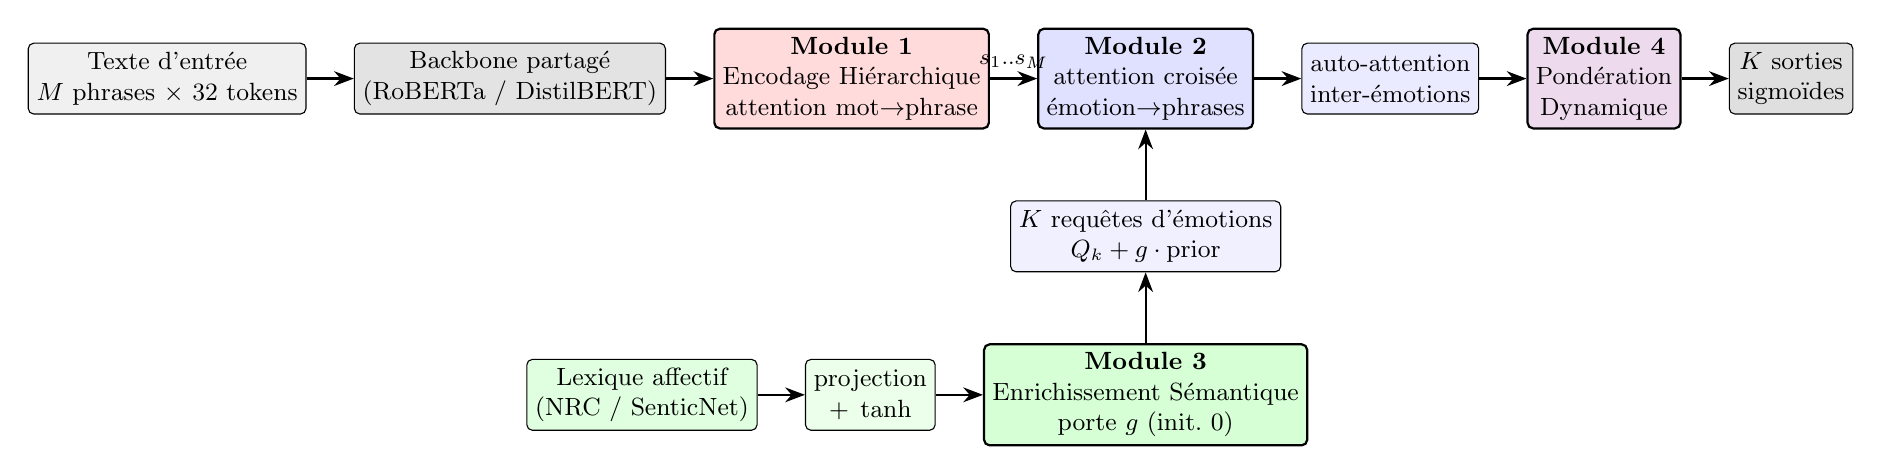
\begin{tikzpicture}[
  font=\small,
  node distance=4mm and 6mm,
  box/.style={draw, rounded corners=2pt, align=center, minimum height=9mm, inner sep=3pt},
  mod/.style={box, thick},
  flow/.style={-{Stealth[length=2.5mm]}, thick}
]
\node[box, fill=gray!12] (input) {Texte d'entrée\\ $M$ phrases $\times$ 32 tokens};
\node[box, fill=gray!22, right=of input] (plm) {Backbone partagé\\ (RoBERTa / DistilBERT)};
\node[mod, fill=red!14, right=of plm] (m1) {\textbf{Module 1}\\ Encodage Hiérarchique\\ attention mot$\to$phrase};
\node[mod, fill=blue!12, right=of m1] (xatt) {\textbf{Module 2}\\ attention croisée\\ émotion$\to$phrases};
\node[box, fill=blue!8, right=of xatt] (inter) {auto-attention\\ inter-émotions};
\node[mod, fill=violet!14, right=of inter] (m4) {\textbf{Module 4}\\ Pondération\\ Dynamique};
\node[box, fill=gray!25, right=of m4] (out) {$K$ sorties\\ sigmoïdes};
\node[box, fill=blue!6, below=9mm of xatt] (q) {$K$ requêtes d'émotions\\ $Q_k + g\cdot\mathrm{prior}$};
\node[mod, fill=green!16, below=9mm of q] (gate) {\textbf{Module 3}\\ Enrichissement Sémantique\\ porte $g$ (init.~0)};
\node[box, fill=green!8, left=of gate] (proj) {projection\\ $+\;\tanh$};
\node[box, fill=green!12, left=of proj] (nrc) {Lexique affectif\\ (NRC / SenticNet)};
\draw[flow] (input) -- (plm);
\draw[flow] (plm) -- (m1);
\draw[flow] (m1) -- node[above, font=\footnotesize\itshape] {$s_1..s_M$} (xatt);
\draw[flow] (xatt) -- (inter);
\draw[flow] (inter) -- (m4);
\draw[flow] (m4) -- (out);
\draw[flow] (q) -- (xatt);
\draw[flow] (nrc) -- (proj);
\draw[flow] (proj) -- (gate);
\draw[flow] (gate) -- (q);
\end{tikzpicture}}
\caption{Architecture de HAKE-MER : quatre modules composables
au-dessus d'un backbone partagé.}
\label{fig:hakemer-archi}
\end{figure}

\section{Module 1 : Encodage Hiérarchique}
\label{sec:conception-m1}

Le texte est segmenté en phrases ($M{=}4$ au plus, 32 tokens par
phrase, bornes fixées au chapitre~\ref{chap:experimentation}), encodées par
le backbone en un seul appel vectorisé. Le module s'inspire de
l'agrégation mot$\to$phrase des réseaux d'attention hiérarchiques
\cite{yang2016}, avec une couche d'\emph{attention additive}
\cite{bahdanau2015}. Pour une phrase de représentations de tokens
$H=(h_1,\dots,h_T)$ et de masque $m$, cette couche calcule :
\begin{equation}
u_t = v^\top \tanh(W h_t), \qquad
\alpha_t = \frac{\exp(u_t)}{\sum_{t'} \exp(u_{t'})}, \qquad
s = \sum_t \alpha_t\, h_t,
\label{eq:attnpool}
\end{equation}
les positions masquées recevant un score $-\infty$ avant le softmax.
On obtient les vecteurs de phrases $s_1,\dots,s_M$. Utilisé seul, le
module applique une seconde attention additive phrase$\to$document et
une tête linéaire partagée ; au sein du modèle complet, ce sont les
vecteurs de phrases qui alimentent le module 2.

\section{Module 2 : Attention Croisée Multi-Émotions}
\label{sec:conception-m2}

Chaque émotion $k$ possède une requête apprise $Q_k \in \mathbb{R}^d$
(initialisée en $\mathcal{N}(0, 0{,}02^2)$). L'attention croisée
multi-têtes (8 têtes, mécanisme Transformer \cite{vaswani2017}) utilise
les requêtes d'émotions comme \emph{queries} et les vecteurs de
phrases comme \emph{keys/values} :
\begin{equation}
r_k = \mathrm{MHA}\big(Q_k,\; [s_1,\dots,s_M],\; [s_1,\dots,s_M]\big),
\label{eq:mha}
\end{equation}
produisant une représentation contextuelle \emph{par émotion} :
chaque émotion « lit » le texte à sa manière. Une couche d'encodeur Transformer \cite{vaswani2017} appliquée sur
l'axe des émotions modélise ensuite leurs interactions (renforcement
ou inhibition mutuels), en complément des approches par chaînes de
classificateurs \cite{read2009classifier}. La tête de classification
est \emph{par étiquette} : chaque émotion a son propre vecteur de
poids, $z_k = w_k^\top r_k + b_k$.

\section{Module 3 : Enrichissement Sémantique}
\label{sec:conception-m3}

Un vecteur affectif de document $c \in \mathbb{R}^{d_c}$ est extrait
d'une ressource externe. Pour le \textbf{NRC Emotion Lexicon}, on
agrège au niveau document un score par émotion de base ($d_c{=}8$,
cadre Plutchik \cite{mohammad2013}), puis on applique une table de
correspondance vers les $K{=}28$ étiquettes GoEmotions (détail du
mapping au chapitre~\ref{chap:experimentation}). Pour
\textbf{SenticNet}, on agrège des scores conceptuels continus issus de
SenticNet~5 \cite{cambria2018senticnet} (primitives et polarité
conceptuelle), regroupés en un vecteur $c$ de dimension $d_c$ fixée au
protocole (chapitre~\ref{chap:experimentation}). Dans les deux cas,
$c$ est projeté, borné, puis injecté dans
les requêtes d'émotions via une \emph{porte apprise} $g$ initialisée à
zéro :
\begin{equation}
\mathrm{prior} = \tanh(W_c\, c), \qquad
\tilde{Q}_k = Q_k + g \cdot \mathrm{prior}.
\label{eq:gate}
\end{equation}
À l'initialisation ($g{=}0$), le module 3 est strictement équivalent
au module 2 : le modèle apprend la quantité de connaissance à
injecter, et la valeur finale $|g|$ mesure directement l'utilisation
de la ressource, une sonde d'interprétabilité intégrée.

\section{Module 4 : Pondération Dynamique}
\label{sec:conception-m4}

Une porte d'intensité par émotion, conditionnée par le contexte
émotionnel global $\bar{r} = \frac{1}{K}\sum_k r_k$ :
\begin{equation}
\gamma_k = \sigma\!\big(W_2\,\mathrm{ReLU}(W_1 [r_k ; \bar{r}]) + b_2\big),
\qquad r_k \leftarrow \gamma_k \cdot r_k,
\label{eq:dyngate}
\end{equation}
avec $b_2$ initialisé à $+3$ (soit $\gamma_k \approx 0{,}95$) : le
module démarre proche de l'identité et apprend à moduler
progressivement l'intensité de chaque émotion selon le texte.

\section{Hypothèses de recherche}
\label{sec:conception-hypotheses}

Le protocole du chapitre~\ref{chap:experimentation} est conçu pour
tester quatre hypothèses. Chacune lie un module à une prédiction
vérifiable sur GoEmotions, sans supposer de gains déjà mesurés :

\begin{itemize}
\item[\textbf{H1.}] La hiérarchie explicite (M1) améliore la
  reconnaissance des émotions rares (F1-macro) en préservant les
  signaux par phrase ;
\item[\textbf{H2.}] La modélisation des interactions entre émotions
  (M2) apporte un gain robuste par rapport à la prédiction
  indépendante ;
\item[\textbf{H3.}] L'injection d'un lexique affectif (M3) aide là où
  la supervision manque, et une ressource \emph{catégorielle} alignée
  sur la taxonomie cible (NRC) est plus efficace qu'une ressource
  \emph{dimensionnelle} abstraite (SenticNet) ;
\item[\textbf{H4.}] Chaque module doit justifier son ajout par
  ablation contrôlée : la plausibilité architecturale ne suffit pas.
\end{itemize}

\section*{Conclusion}
\addcontentsline{toc}{section}{Conclusion}
Ce chapitre a présenté la conception de HAKE-MER : quatre modules
composables répondant aux limitations L1 à L3, avec deux portes apprises
et interprétables (connaissance externe, intensité). Le
chapitre~\ref{chap:experimentation} précise le protocole d'ablation à
budget constant, les backbones et les analyses qui permettront de
valider ou d'infirmer H1 à H4.

        \clearpage

        \chapter{Expérimentations et résultats}
\label{chap:experimentation}

\section*{Introduction}
\addcontentsline{toc}{section}{Introduction}
Ce chapitre évalue HAKE-MER sur GoEmotions par une ablation
cumulative à protocole strictement constant, complétée par une
comparaison des ressources de connaissances externes et par des
analyses qualitative et d'erreur. Les hypothèses H1 à H4 du
chapitre 3 y sont confrontées aux résultats.

\section{Cadre expérimental}
\label{sec:expe-cadre}

\subsection{Jeu de données}
Toutes les expériences utilisent GoEmotions \cite{demszky2020}
(configuration \emph{simplified}) : 43\,410 exemples d'entraînement,
5\,426 de validation et 5\,427 de test, 27 émotions plus la classe
neutre ($K{=}28$), en multi-étiquettes. L'analyse exploratoire
éclaire trois choix : le \textbf{déséquilibre} (\emph{neutral} :
14\,219 occurrences contre 77 pour \emph{grief}, rapport de 185)
impose le F1-macro comme métrique décisive ; la
\textbf{multi-étiquette} est réelle (16{,}4\,\% des exemples portent
au moins deux émotions ; paires fréquentes :
\emph{admiration}+\emph{gratitude} 279,
\emph{anger}+\emph{annoyance} 269) ; la \textbf{structure} (longueur
moyenne 19 tokens, 42{,}2\,\% de textes multi-phrases) justifie les
bornes du prétraitement hiérarchique ($M{=}4$ phrases de 32 tokens —
à 20 tokens, 24{,}1\,\% des exemples étaient tronqués contre
1{,}8\,\% à 32).

\subsection{Protocole}
Toutes les configurations partagent : 5~époques (budget fixé après
constat d'un plateau au-delà), graine aléatoire 42, taille de lot 24
(32 pour la ligne de base plate), précision mixte sur GPU~T4, et les
mêmes métriques : F1-micro, \textbf{F1-macro} (métrique de référence,
seule sensible aux émotions rares), correspondance exacte et mAP.
L'architecture est implémentée comme une classe unique à indicateurs
d'activation : les configurations comparées ne diffèrent que par les
modules activés.

\section{Choix des backbones}
\label{sec:expe-backbones}

Un comparatif préliminaire de quatre encodeurs à protocole identique
(tableau~\ref{tab:backbones}) a guidé le choix : RoBERTa-base
\cite{liu2019roberta} domine sur F1-macro et mAP ; DistilBERT-base
\cite{sanh2019distilbert} offre le meilleur compromis
coût/performance ; ALBERT \cite{lan2020albert}, malgré son faible
nombre de paramètres, est le plus lent à entraîner et le plus faible
en F1-macro. La suite rapporte systématiquement DistilBERT \emph{et}
RoBERTa.

\begin{table}[H]
\centering
\small
\begin{tabular}{lccccc}
\toprule
Modèle & Params & Temps (5 ép., T4) & F1-micro & F1-macro & mAP\\
\midrule
RoBERTa-base \cite{liu2019roberta}       & 125M & 805\,s  & \textbf{0,588} & \textbf{0,488} & \textbf{0,516}\\
BERT-base \cite{devlin2019}              & 110M & 787\,s  & 0,579 & 0,480 & 0,500\\
DistilBERT-base \cite{sanh2019distilbert}& 67M  & \textbf{415\,s} & 0,579 & 0,475 & 0,498\\
ALBERT-base-v2 \cite{lan2020albert}      & 12M  & 1\,020\,s & 0,584 & 0,467 & 0,491\\
\bottomrule
\end{tabular}
\caption{Comparatif préliminaire des encodeurs sur GoEmotions (test),
protocole identique.}
\label{tab:backbones}
\end{table}

\section{Ablation cumulative}
\label{sec:expe-ablation}

Le tableau~\ref{tab:ablation} présente le résultat central du
travail : l'ablation cumulative des quatre modules, sur les deux
backbones.

\begin{table}[H]
\centering
\small
\begin{tabular}{l cccc cccc}
\toprule
& \multicolumn{4}{c}{RoBERTa-base} & \multicolumn{4}{c}{DistilBERT-base}\\
\cmidrule(lr){2-5}\cmidrule(lr){6-9}
Configuration & F1-mi & F1-ma & Exact & mAP & F1-mi & F1-ma & Exact & mAP\\
\midrule
Ligne de base (PLM affiné)      & 0,584 & 0,476 & \textbf{0,475} & 0,504 & \textbf{0,590} & 0,459 & \textbf{0,473} & 0,502\\
M1 (hiérarchique)               & 0,575 & 0,509 & 0,461 & 0,512 & 0,558 & 0,438 & 0,448 & 0,487\\
M1+M2 (attention croisée)       & \textbf{0,588} & 0,510 & 0,466 & 0,520 & 0,586 & 0,480 & 0,468 & 0,505\\
M1+M2+M3 (enrichissement)       & 0,585 & \textbf{0,523} & 0,458 & \textbf{0,532} & 0,586 & \textbf{0,499} & 0,467 & 0,511\\
M1+M2+M3+M4 (complet)           & 0,586 & 0,496 & 0,461 & 0,520 & 0,584 & 0,485 & 0,463 & \textbf{0,512}\\
\bottomrule
\end{tabular}
\caption{Ablation cumulative de HAKE-MER sur GoEmotions (test),
protocole constant (5~époques, graine~42). Les chiffres RoBERTa
proviennent d'une unique session entraînant les cinq configurations
(modèle final) ; les chiffres DistilBERT de runs par module au même
budget (meilleur point de contrôle sur validation).}
\label{tab:ablation}
\end{table}

\subsection{Lecture des résultats}

\textbf{Le F1-macro progresse à chaque module jusqu'à M3.} Sur
RoBERTa : $0{,}476 \to 0{,}509$ (M1) $\to 0{,}510$ (M2)
$\to \mathbf{0{,}523}$ (M3), soit $\mathbf{+0{,}047}$ au-dessus de la
ligne de base — sur la métrique qui capture les émotions rares,
l'objectif central du sujet. Le mAP suit la même trajectoire (0,504
$\to$ 0,532). L'hypothèse H1 est validée \emph{conditionnellement au
backbone} : la hiérarchie seule améliore nettement RoBERTa
($+0{,}033$ de F1-macro) mais \emph{dégrade} DistilBERT ($-0{,}021$).

\textbf{L'attention croisée corrige la hiérarchie seule (H2).} Sur
les deux backbones, M2 restaure le F1-micro que M1 dégradait
(DistilBERT : $0{,}558 \to 0{,}586$) tout en maintenant ou améliorant
le F1-macro — cohérent avec les co-occurrences mesurées.

\textbf{Le module 4 ne justifie pas son ajout (H4).} La pondération
dynamique fait reculer le F1-macro sur les deux backbones
($0{,}523 \to 0{,}496$ sur RoBERTa). Ce résultat négatif, assumé,
illustre la nécessité de l'ablation contrôlée : une composante
plausible peut ne rien apporter. La meilleure configuration retenue
est donc \textbf{M1+M2+M3}.

\section{Comparaison des connaissances externes}
\label{sec:expe-ressources}

L'hypothèse H3 est testée à architecture et budget fixés, en ne
faisant varier que la ressource injectée par la porte du module~3
(tableau~\ref{tab:ressources}).

\begin{table}[H]
\centering
\small
\begin{tabular}{llccccc}
\toprule
Backbone & Ressource (type) & F1-micro & F1-macro & Exact & mAP & porte $g$\\
\midrule
DistilBERT & NRC (lexical, 10-d)          & 0,586 & \textbf{0,499} & 0,467 & \textbf{0,511} & $+0{,}029$\\
DistilBERT & SenticNet (conceptuel, 5-d)  & 0,587 & 0,486 & 0,470 & 0,507 & $+0{,}027$\\
RoBERTa    & NRC (lexical, 10-d)          & \textbf{0,595} & \textbf{0,492} & \textbf{0,479} & \textbf{0,525} & $-0{,}027$\\
RoBERTa    & SenticNet (conceptuel, 5-d)  & 0,588 & 0,461 & 0,471 & 0,510 & $+0{,}023$\\
\bottomrule
\end{tabular}
\caption{Module 3 avec deux ressources de connaissance, à
architecture et budget fixés. La porte $g$ non nulle atteste
l'utilisation effective de la connaissance.}
\label{tab:ressources}
\end{table}

Le NRC \cite{mohammad2013} domine SenticNet
\cite{cambria2018senticnet} sur le F1-macro pour les deux backbones
($+0{,}013$ DistilBERT, $+0{,}031$ RoBERTa) : les catégories
d'émotions du lexique s'alignent directement sur les étiquettes de
GoEmotions, là où les dimensions abstraites de SenticNet exigeraient
une mise en correspondance que l'injection par biais ne fournit pas.
H3 est validée : le rendement de la connaissance dépend de
l'\emph{alignement taxonomique}.

\section{Analyse qualitative}
\label{sec:expe-qualitatif}

Le suivi d'exemples de classes rares, configuration par
configuration (tableau~\ref{tab:qualitatif}), illustre le rôle de
chaque module : la hiérarchie corrige \emph{relief} là où la ligne de
base prédit \emph{sadness} ; l'attention croisée retrouve le couple
complet \emph{joy}+\emph{surprise}. À l'inverse, \emph{grief} n'est
détectée par aucune configuration (6 exemples de test seulement) —
l'illustration extrême du problème des classes quasi vides.

\begin{table}[H]
\centering
\footnotesize
\begin{tabular}{p{4.6cm}p{2.2cm}p{2.0cm}p{2.0cm}p{2.4cm}}
\toprule
Exemple (extrait) & Vraies étiquettes & Ligne de base & M1 & M1+M2(+M3)\\
\midrule
« Resetting a dislocated knee hurts... feels a lot better immediately after » & relief & sadness & \textbf{relief} & \textbf{relief}\\
« A surprise turn of events! I'm so glad... » & joy, surprise & surprise & admiration & \textbf{joy, surprise}\\
« [NAME] death is just so... senseless. Why? WHY??? » & grief & sadness & disappointment & sadness\\
\bottomrule
\end{tabular}
\caption{Évolution des prédictions sur des exemples de classes rares
(backbone RoBERTa).}
\label{tab:qualitatif}
\end{table}

\section{Analyse d'erreur}
\label{sec:expe-erreur}

Sur le modèle complet (RoBERTa), les confusions sont dominées par la
frontière avec \emph{neutral} : les paires les plus fréquentes
(étiquette vraie manquée $\to$ étiquette prédite à la place) sont
neutral$\to$curiosity (69), annoyance$\to$neutral (64) et
approval$\to$neutral (63) — le modèle peine à départager les émotions
\emph{subtiles} du neutre, davantage qu'à confondre deux émotions
marquées. Le F1 par classe confirme la structure attendue : minimal
sur \emph{grief} (0,00), \emph{relief} (0,13), \emph{realization}
(0,26) et \emph{nervousness} (0,30), maximal sur \emph{gratitude}
(0,92), \emph{amusement} (0,82) et \emph{love} (0,80) — classes
fréquentes aux indices lexicaux saillants.

\section{Positionnement par rapport à la littérature}
\label{sec:expe-sota}

À titre indicatif, le F1-macro obtenu par la meilleure configuration
(M1+M2+M3, RoBERTa) est rapproché du chiffre de référence publié par
les auteurs du jeu de données GoEmotions \cite{demszky2020}, qui
rapportent un F1-macro de 0,46 et un F1-micro de 0,51 pour un
classifieur BERT-base affiné sur la taxonomie complète à 28 classes
(tableau~\ref{tab:sota}).

\begin{table}[H]
\centering
\small
\begin{tabular}{llcc}
\toprule
Étude & Modèle & F1-micro & F1-macro\\
\midrule
Demszky et al. (2020) \cite{demszky2020} & BERT-base & 0,51 & 0,46\\
Notre travail (ce mémoire) & HAKE-MER M1+M2+M3 (RoBERTa) & \textbf{0,585} & \textbf{0,523}\\
\bottomrule
\end{tabular}
\caption{Repère indicatif par rapport au chiffre de référence publié
sur GoEmotions. Comparaison non strictement contrôlée : le protocole
d'entraînement original (nombre d'époques, taille de séquence,
recherche d'hyperparamètres) n'est pas reproduit à l'identique ; seule
la comparaison interne par ablation (tableau~\ref{tab:ablation}) isole
rigoureusement l'apport des modules de HAKE-MER.}
\label{tab:sota}
\end{table}

Cet écart positif est cohérent avec les gains internes mesurés par
ablation, mais ne constitue pas une preuve de supériorité au sens
strict : contrairement au protocole d'ablation cumulative de ce
chapitre, où seul le budget d'entraînement est maintenu constant, la
configuration exacte de \cite{demszky2020} (nombre d'époques, longueur
de séquence, recherche d'hyperparamètres) n'a pas été reproduite à
l'identique. Ce repère situe néanmoins HAKE-MER par rapport au point
d'ancrage le plus largement cité de la littérature sur GoEmotions,
sans remplacer la comparaison contrôlée qui reste la preuve principale
de ce mémoire.

\section{Leçons méthodologiques}
\label{sec:expe-lecons}

Trois incidents résolus en cours de développement méritent d'être
consignés, car chacun modifiait matériellement les conclusions :

\begin{itemize}
\item \textbf{Troncature du prétraitement.} La première borne de
  20 tokens/phrase tronquait 18{,}7\,\% des exemples et faisait
  passer le module 1 \emph{sous} la ligne de base — l'écart mesurait
  le prétraitement, pas l'architecture. Borne recalibrée à 32 tokens.
\item \textbf{Échelle d'initialisation.} Les requêtes d'émotions
  initialisées en $\mathcal{N}(0,1)$ produisaient une perte initiale
  de 1,86 (contre 0,18 après correction en
  $\mathcal{N}(0,0{,}02^2)$).
\item \textbf{Équité des budgets.} Comparer des configurations à
  budgets d'entraînement différents inversait certaines conclusions ;
  d'où le protocole à budget strictement constant.
\end{itemize}

\section*{Conclusion}
\addcontentsline{toc}{section}{Conclusion}
L'ablation cumulative établit que la configuration M1+M2+M3 sur
RoBERTa atteint un F1-macro de 0,523, soit $+0{,}047$ au-dessus du
PLM affiné, le gain se concentrant sur les émotions rares ; le NRC
surpasse SenticNet à architecture fixée ; et le module 4 ne justifie
pas son ajout. Les analyses qualitative et d'erreur situent les
limites restantes : classes quasi vides et frontière avec le neutre.

        \clearpage

        \chapter{Recommandations et perspectives}
\label{chap:perspectives}

\section*{Introduction}
\addcontentsline{toc}{section}{Introduction}
Ce chapitre recueille des recommandations méthodologiques pour la
détection multi-étiquettes des émotions et ouvre des perspectives de
prolongement, en lien avec le protocole du
chapitre~\ref{chap:experimentation}.

\section{Principes méthodologiques}
\label{sec:persp-enseignements}

Quatre principes guideront l'évaluation de HAKE-MER et, plus
généralement, tout travail sur GoEmotions :
\begin{itemize}
\item \textbf{Multi-backbone.} L'effet d'un module architectural peut
      dépendre de la capacité de l'encodeur ; conclure à partir d'un
      seul PLM est risqué.
\item \textbf{Contrôle du prétraitement.} Troncature, segmentation en
      phrases et initialisation des têtes peuvent masquer ou imiter
      un gain architectural.
\item \textbf{Métriques par classe.} Le F1-macro seul ne suffit pas :
      les classes rares et la frontière avec \emph{neutral} doivent
      être inspectées explicitement.
\item \textbf{Comparaisons externes prudentes.} Se reporter à la
      littérature n'a de sens qu'avec un protocole comparable ou une
      discussion honnête des écarts.
\end{itemize}

\section{Recommandations pratiques (après expériences)}
\label{sec:persp-recommandations}

Une fois les ablations menées, la configuration retenue devra être
justifiée par les métriques \emph{et} par le coût (temps GPU,
paramètres). Le plan prévoit de comparer M1+M2+M3
avec NRC sur RoBERTa et DistilBERT, puis de tester M4 seulement si
M1--M3 apportent un gain mesurable.

\section{Perspectives de recherche}
\label{sec:persp-recherche}

\begin{itemize}
\item \textbf{Traitement du déséquilibre.} Pertes focales ou
      repondérées, seuils par émotion ;
\item \textbf{Enrichissement sémantique.} Au-delà de NRC/SenticNet,
      graphes de connaissances (ConceptNet, ressources affectives) et
      fusion adaptative par émotion ;
\item \textbf{Validation externe.} SemEval-2018 Tâche~1, plusieurs
      graines aléatoires ;
\item \textbf{Émotions implicites.} Ressources de bon sens (ATOMIC,
      COMET) ;
\item \textbf{LLM.} Positionner HAKE-MER par rapport aux modèles
      généralistes et aux LLM affectifs spécialisés lorsque des
      baselines reproductibles sont disponibles.
\end{itemize}

\section*{Conclusion}
\addcontentsline{toc}{section}{Conclusion}
Les perspectives ci-dessus prolongent le sujet au-delà du protocole
détaillé au chapitre~\ref{chap:experimentation}.

        \clearpage

        \chapter*{Conclusion générale et Perspectives}
\addcontentsline{toc}{chapter}{Conclusion générale et Perspectives}
\markboth{Conclusion générale et Perspectives}{}

Ce mémoire vise la détection des émotions multiples dans les textes,
une tâche où les approches mono-étiquette et les représentations
textuelles plates peinent à refléter la cooccurrence des affects et
le déséquilibre sévère des classes sur des corpus tels que
GoEmotions \cite{demszky2020}.

L'architecture \textbf{HAKE-MER} a été conçue de manière modulaire
afin de mesurer, à protocole constant sur GoEmotions, l'apport de
chaque brique. Les expériences menées sur DistilBERT-base (trois
graines) montrent que \textbf{M2} (attention croisée et têtes par
émotion) porte le gain principal en F1-macro test ($\approx 0{,}505$),
que \textbf{M1} seul sous-performe une baseline PLM flat
($\approx 0{,}486$), et que \textbf{M3} (NRC ou SenticNet) n'améliore
pas de façon robuste la macro par rapport à M1+M2 (H3 tranchée au
chapitre~\ref{chap:experimentation}). Il reste à évaluer \textbf{M4}
(H4) sur la pile M3 retenue, puis à compléter l'analyse par classe et
les exemples qualitatifs.

Les prolongements possibles (autres corpus, graphes de connaissances,
modèles généralistes) sont discutés au chapitre~\ref{chap:perspectives}.

        \clearpage
        
        \printbibliography[heading=bibintoc]
        
    %     \chapter*{Annexes}
\addcontentsline{toc}{chapter}{Annexes}
\markboth{Annexes}{}
\stepcounter{chapter}
\addtocontents{lot}{\vspace{3.8mm}}
\addtocontents{lof}{\vspace{3.8mm}}

% Auto-generated from campaign aggregate; do not hand-edit rows.
\section*{Annexe A.~F1 test par émotion (DistilBERT, 3 graines)}
\addcontentsline{toc}{section}{Annexe A.~F1 test par émotion}

Tableau complet complétant le tableau~\ref{tab:expe-per-class-f1} du
chapitre~\ref{chap:experimentation} (même protocole, moyenne $\pm$
écart-type sur les graines $42$, $123$, $456$).

{\small
\renewcommand{\arraystretch}{1.15}
\begin{longtable}{|l|r|c|c|c|}
\hline
\textbf{Émotion} & \textbf{Support} & \textbf{Step~0} & \textbf{+M1} & \textbf{+M1+M2} \\
\hline
\endhead
admiration & 504 & $0{,}684 \pm 0{,}010$ & $0{,}675 \pm 0{,}010$ & $0{,}686 \pm 0{,}003$ \\
\hline
amusement & 264 & $0{,}820 \pm 0{,}006$ & $0{,}792 \pm 0{,}022$ & $0{,}817 \pm 0{,}001$ \\
\hline
anger & 198 & $0{,}485 \pm 0{,}012$ & $0{,}449 \pm 0{,}015$ & $0{,}486 \pm 0{,}016$ \\
\hline
annoyance & 320 & $0{,}309 \pm 0{,}010$ & $0{,}295 \pm 0{,}023$ & $0{,}358 \pm 0{,}013$ \\
\hline
approval & 351 & $0{,}384 \pm 0{,}018$ & $0{,}342 \pm 0{,}018$ & $0{,}387 \pm 0{,}009$ \\
\hline
caring & 135 & $0{,}416 \pm 0{,}011$ & $0{,}349 \pm 0{,}003$ & $0{,}400 \pm 0{,}014$ \\
\hline
confusion & 153 & $0{,}449 \pm 0{,}008$ & $0{,}410 \pm 0{,}014$ & $0{,}437 \pm 0{,}015$ \\
\hline
curiosity & 284 & $0{,}479 \pm 0{,}021$ & $0{,}497 \pm 0{,}015$ & $0{,}512 \pm 0{,}021$ \\
\hline
desire & 83 & $0{,}445 \pm 0{,}018$ & $0{,}412 \pm 0{,}025$ & $0{,}511 \pm 0{,}016$ \\
\hline
disappointment & 151 & $0{,}270 \pm 0{,}013$ & $0{,}233 \pm 0{,}013$ & $0{,}286 \pm 0{,}014$ \\
\hline
disapproval & 267 & $0{,}384 \pm 0{,}026$ & $0{,}351 \pm 0{,}013$ & $0{,}380 \pm 0{,}007$ \\
\hline
disgust & 123 & $0{,}489 \pm 0{,}005$ & $0{,}475 \pm 0{,}027$ & $0{,}462 \pm 0{,}006$ \\
\hline
embarrassment & 37 & $0{,}497 \pm 0{,}017$ & $0{,}433 \pm 0{,}031$ & $0{,}407 \pm 0{,}040$ \\
\hline
excitement & 103 & $0{,}430 \pm 0{,}019$ & $0{,}392 \pm 0{,}025$ & $0{,}434 \pm 0{,}008$ \\
\hline
fear & 78 & $0{,}651 \pm 0{,}002$ & $0{,}659 \pm 0{,}007$ & $0{,}644 \pm 0{,}017$ \\
\hline
gratitude & 352 & $0{,}920 \pm 0{,}003$ & $0{,}905 \pm 0{,}003$ & $0{,}920 \pm 0{,}005$ \\
\hline
grief & 6 & $0{,}000 \pm 0{,}000$ & $0{,}000 \pm 0{,}000$ & $0{,}257 \pm 0{,}040$ \\
\hline
joy & 161 & $0{,}624 \pm 0{,}015$ & $0{,}577 \pm 0{,}012$ & $0{,}617 \pm 0{,}020$ \\
\hline
love & 238 & $0{,}798 \pm 0{,}006$ & $0{,}771 \pm 0{,}006$ & $0{,}797 \pm 0{,}017$ \\
\hline
nervousness & 23 & $0{,}392 \pm 0{,}020$ & $0{,}387 \pm 0{,}066$ & $0{,}302 \pm 0{,}035$ \\
\hline
optimism & 186 & $0{,}555 \pm 0{,}018$ & $0{,}481 \pm 0{,}018$ & $0{,}550 \pm 0{,}019$ \\
\hline
pride & 16 & $0{,}406 \pm 0{,}037$ & $0{,}343 \pm 0{,}041$ & $0{,}447 \pm 0{,}050$ \\
\hline
realization & 145 & $0{,}228 \pm 0{,}015$ & $0{,}222 \pm 0{,}006$ & $0{,}244 \pm 0{,}008$ \\
\hline
relief & 11 & $0{,}158 \pm 0{,}126$ & $0{,}051 \pm 0{,}073$ & $0{,}398 \pm 0{,}097$ \\
\hline
remorse & 56 & $0{,}628 \pm 0{,}002$ & $0{,}631 \pm 0{,}013$ & $0{,}647 \pm 0{,}018$ \\
\hline
sadness & 156 & $0{,}579 \pm 0{,}013$ & $0{,}560 \pm 0{,}008$ & $0{,}575 \pm 0{,}013$ \\
\hline
surprise & 141 & $0{,}546 \pm 0{,}008$ & $0{,}515 \pm 0{,}019$ & $0{,}550 \pm 0{,}004$ \\
\hline
neutral & 1787 & $0{,}628 \pm 0{,}013$ & $0{,}620 \pm 0{,}012$ & $0{,}629 \pm 0{,}005$ \\
\hline

\end{longtable}
}


\newpage
%===================== ANNEXE ENTREPRISE =====================%
\section*{Annexe B.~Entreprise}
\addcontentsline{toc}{section}{Annexe B.~Entreprise}

\addcontentsline{lof}{figure}{Annexe B.1~~~Logo d'entreprise}

La figure annexe B.1 présente le logo entreprise.
\begin{figure}[htpb]
    \centering
    \frame{
\includegraphics[width=0.45\columnwidth]{Logo_Entreprise}}
    {\\\textbf{Figure annexe B.1:} Logo d'entreprise}
\end{figure}

    %     \clearpage

     % \backmatter
     %    \input{./tpl/resume}
    
\end{document}